\begin{surferPage}{Ein Doppelkegel}
 Eine Fläche heißt nicht-singulär oder glatt, wenn sie, anschaulich gesagt,
    keine spitzen Stellen (Singularitäten genannt) hat, z.B.\ eine Kugel, 
    ein Torus (1.\ bzw.\ 2.\ Bild von links):
    \vspace{-0.2cm}
    \begin{center}
      \begin{tabular}{@{}c@{}c@{}c@{}c@{}}
        \begin{tabular}{@{}c}
          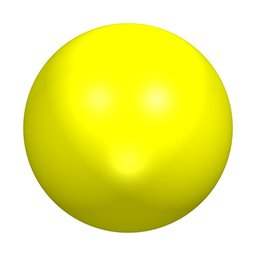
\includegraphics[width=1.1cm]{../../common/images/kugel}
        \end{tabular}
        &
        \begin{tabular}{@{}c}
          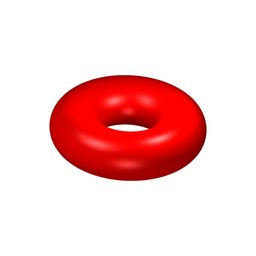
\includegraphics[width=1.1cm]{../../common/images/torus}
        \end{tabular}
        &
        \begin{tabular}{c@{}}
          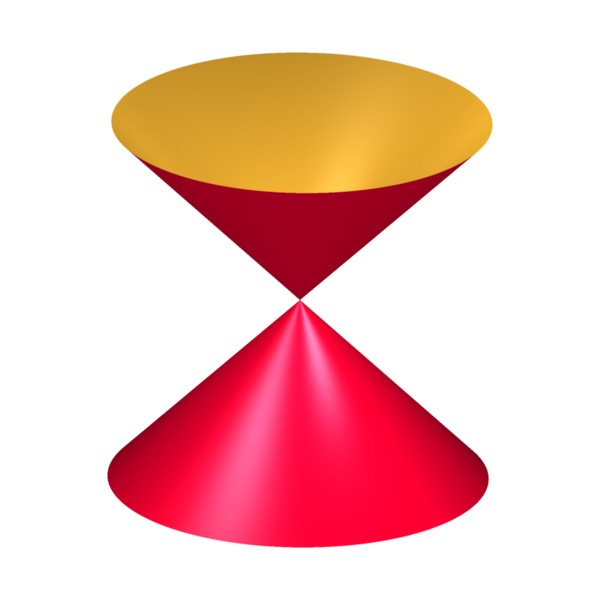
\includegraphics[width=1.1cm]{../../common/images/kegel}
        \end{tabular}
        &
        \begin{tabular}{c@{}}
          
\includegraphics[width=1.1cm]{../../common/images/A2pm_ill}
        \end{tabular}
      \end{tabular}
    \end{center}
    \vspace*{-0.4em}
    Der Doppelkegel (auch Singularität vom Typ $A_1^{+-}$) ist die einfachste
    Singularität:
    stört man seine Gleichung 
    \[x^2+y^2-z^2=0\]
    leicht, so wird die Fläche glatt.
    Die Bilder unten zeigen z.B.\ Flächen mit der Gleichung 
    \[x^2+y^2-z^2=a\]
    für die Werte $a=-\frac12$, $a=0$, $a=\frac12$:
    % 
    \begin{center}
      \vspace*{-0.4em}
      \begin{tabular}{@{}c@{\quad}c@{\quad}c@{}}
        \begin{tabular}{@{}c@{}}
          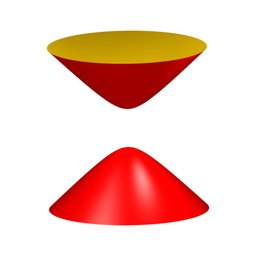
\includegraphics[width=1.2cm]{../../common/images/A1pm_0}
        \end{tabular}
        &
        \begin{tabular}{@{}c@{}}
          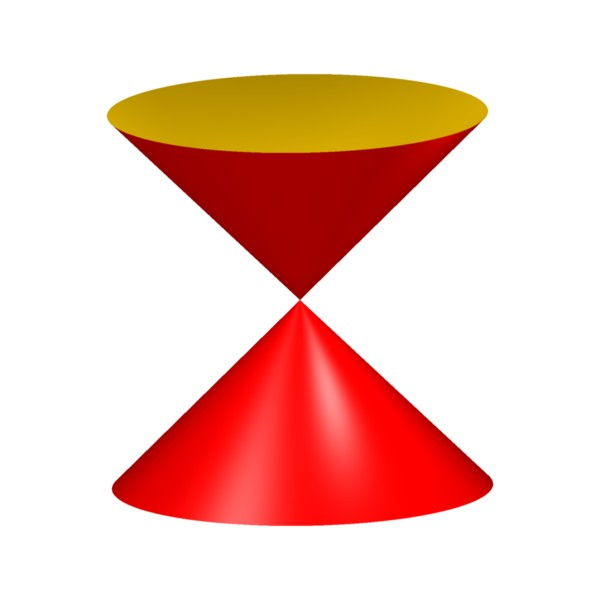
\includegraphics[width=1.2cm]{../../common/images/A1pm_1}
        \end{tabular}
        &
        \begin{tabular}{@{}c@{}}
          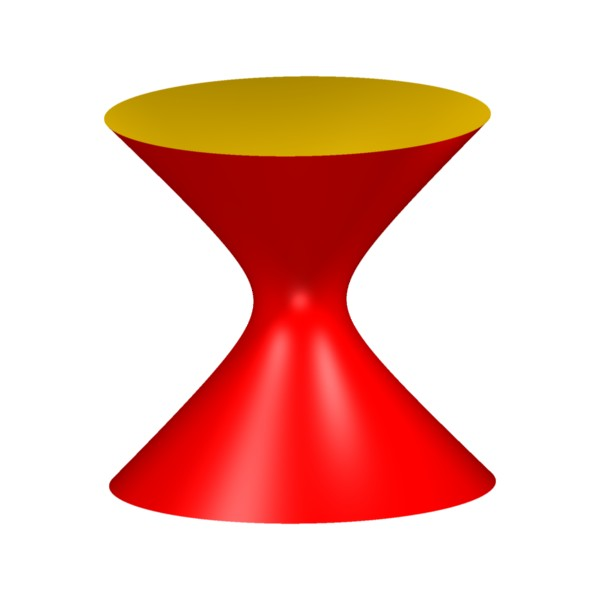
\includegraphics[width=1.2cm]{../../common/images/A1pm_2}
        \end{tabular}
      \end{tabular}
    \end{center}
    \vspace*{-0.4em}
    Wir werden auf den nächsten Seiten sehen, dass man kompliziertere
    Singularitäten oft so stören kann, dass sich mehrere Doppelkegel bilden. 
\end{surferPage}
